
\documentclass[11pt,a4paper]{article}

\usepackage[utf8]{inputenc}
\usepackage[T1]{fontenc}
\usepackage{amsmath}
\usepackage{amssymb}
\usepackage{booktabs}
\usepackage{graphicx}
\usepackage{geometry}
\geometry{margin=2.5cm}

\title{Mathematical Formulation and Metrics}
\author{Enviroment Research Project}
\date{}

\begin{document}

\maketitle

\section{Performance Metrics}

\subsection{Latency}

Latency is defined as the execution time
of an individual operation:

\begin{equation}
L_i =
\underbrace{t_{\mathrm{end},i}}_{\text{End time}}
-
\underbrace{t_{\mathrm{start},i}}_{\text{Start time}}
\label{eq:latency}
\end{equation}

The mean latency is:

\begin{equation}
\overline{L} =
\frac{1}{n}\sum_{i=1}^{n}L_i
\label{eq:mean_latency}
\end{equation}

\subsection{Tail Latency}

The 95th and 99th percentiles are:

\begin{align}
p_{95} &= Q_{0.95}(\mathbf{L}),\\
p_{99} &= Q_{0.99}(\mathbf{L}).
\end{align}

\subsection{Throughput}

Throughput is the number of completed
operations per unit time:

\begin{equation}
R = \frac{N}{T}
\end{equation}

\subsection{Bootstrap Confidence Interval}

A percentile bootstrap confidence interval is:

\begin{equation}
CI_{95\%} =
\left[
Q_{0.025}(\hat{\theta}^{*}),
Q_{0.975}(\hat{\theta}^{*})
\right]
\label{eq:bootstrap_ci}
\end{equation}

\subsection{Relative Speedup}

The speedup ratio is defined as:

\begin{equation}
S =
\frac{\overline{L}_{\mathrm{baseline}}}
     {\overline{L}_{\mathrm{proposed}}}
\label{eq:speedup}
\end{equation}

For the evaluated synthetic workload:

\begin{equation}
S = \frac{2.275}{30.787}
\approx 0.0739
\end{equation}

Since $S < 1$, the proposed implementation
is slower than the baseline.

\section{Notation Table}

\begin{table}[htbp]
\centering
\caption{Mathematical Notation}
\label{tab:notation}
\begin{tabular}{llll}
\toprule
Symbol & Type & Description & Unit \\
\midrule
$L_i$ & Scalar & Latency of run $i$ & ms \\
$n$ & Scalar & Measured runs & count \\
$\overline{L}$ & Scalar & Mean latency & ms \\
$S$ & Scalar & Speedup ratio & -- \\
$R$ & Scalar & Throughput & ops/s \\
$\mathbf{L}$ & Vector & Latency values & ms \\
$\mathbf{X}$ & Matrix & Input data & varies \\
$\mathcal{D}$ & Set & Dataset & -- \\
$\mathcal{I}$ & Set & Run indices & -- \\
\bottomrule
\end{tabular}
\end{table}

\section{Experimental Notes}

Warm-up executions are excluded from
performance measurements.

The comparison uses 120 measured runs
per implementation on a synthetic
dataset of 1,848 rows.

Bootstrap uncertainty estimates use
2,000 resamples with random seed 42.
\clearpage
% ==============================================================================
% reports/tables.tex — Publication Tables in LaTeX booktabs format
% SYNTHETIC DATA -- pipeline test only
% ==============================================================================

% --- Table 1: Corpus Descriptives ---

% Table 1: Corpus Descriptives

\begin{table}[htbp]
\centering
\small

\caption{Corpus Characteristics Before and After
Quality Filtration (Synthetic Data)}

\label{tab:corpus_descriptives}

\begin{tabular}{lrrrrr}
\toprule

\textbf{Sample Stage} &
\textbf{Records} &
\textbf{Replika} &
\textbf{Character.AI} &
\textbf{Words} &
\textbf{Excluded} \\

\midrule

Raw Synthetic Pool & 360 & 188 & 172 & 54,435 & -- \\

\quad Excluded: $w < 100$ words
& 152 & 83 & 69 & -- & 152 \\

\quad Excluded: $w > 3000$ words
& 1 & 0 & 1 & -- & 1 \\

\quad Excluded: Sessions $\notin [1,21]$
& 4 & 2 & 2 & -- & 4 \\

\quad Excluded: Student unknown
& 56 & 28 & 28 & -- & 56 \\

\midrule

\textbf{Final Analysis Dataset}
& \textbf{171} & \textbf{90}
& \textbf{81} & \textbf{33,754}
& \textbf{189} \\

\quad Group 1: $<1$ month
& 38 & 17 & 21 & 7,593 & -- \\

\quad Group 2: $1$--$3$ months
& 57 & 32 & 25 & 12,175 & -- \\

\quad Group 3: $>3$ months
& 76 & 41 & 35 & 13,986 & -- \\

\bottomrule
\end{tabular}

\par\smallskip
{\footnotesize\emph{Note:}
Exclusion criteria may overlap; category counts
should not be summed to obtain total exclusions.
All data are synthetic.}

\end{table}



% --- Table 2: RQ2 Results ---
\begin{table}[htbp]
\centering
\small
\caption{Emotional Dependence Marker Frequency
($F_i$) by Usage Duration
(SYNTHETIC DATA -- pipeline test only)}
\label{tab:rq2_results}

\begin{tabular}{lccc}
\toprule
Group & $n$ & Mean $\pm$ SD &
Median ($p_{25}$--$p_{75}$) \\
\midrule
$<1$ month ($G_1$) & 38 &
$11.03 \pm 7.81$ & $10.69$ ($6.03$--$15.61$) \\

$1$--$3$ months ($G_2$) & 57 &
$13.52 \pm 9.36$ & $11.70$ ($7.30$--$19.32$) \\

$>3$ months ($G_3$) & 76 &
$24.59 \pm 22.77$ & $20.78$ ($9.31$--$33.24$) \\
\bottomrule
\end{tabular}

\vspace{0.5em}

\begin{tabular}{ll}
\toprule
Statistical Test & Result \\
\midrule
Mann--Whitney $U$ ($G_3 > G_1$) &
$U = 2079.5$, $p = 6.73 \times 10^{-5}$ \\

Cliff's delta (95\% CI) &
$\delta = 0.440$ $[0.250, 0.614]$ \\

Kruskal--Wallis &
$H = 19.15$, $p = 6.95 \times 10^{-5}$ \\

Jonckheere--Terpstra &
$J = 6206.5$, $Z = 4.35$,
$p = 6.67 \times 10^{-6}$ \\
\bottomrule
\end{tabular}

\end{table}

% --- Figure Subcaption LaTeX Environment ---
\begin{figure}[t]
\centering
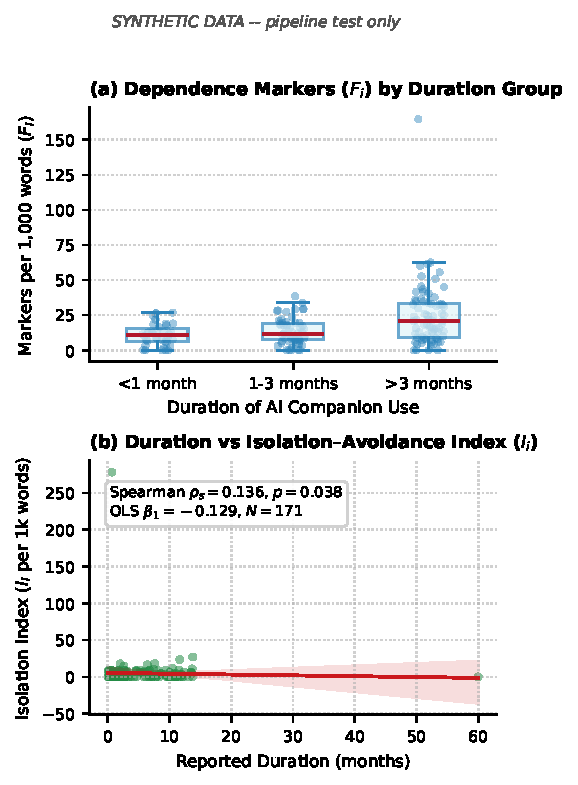
\includegraphics[width=\columnwidth]{figures/study/study_results.pdf}
\caption{Quantitative findings for emotional dependence and social avoidance across duration strata (\textit{SYNTHETIC DATA -- pipeline test only}). (a) Boxplots with overlaid strip observations show dependence markers per 1,000 words ($F_i$) across three usage durations. Whiskers span $1.5 \times \text{IQR}$; central line represents the group median. (b) Bivariate relationship between interaction duration (months) and the isolation--avoidance index ($I_i$). The solid red line indicates the linear OLS fit; shaded band shows the 95\% bootstrap confidence interval ($B = 1,000$ resamples).}
\label{fig:study_results}
\end{figure}

\end{document}
